随着时代的发展和项目变得越来越复杂,人们创造了一系列新的代码特性,其中一些特性在C++11和C++17中被引入,
在不熟悉这些特性的人看来,这些代码看上去显得十分无厘头,甚至有些难以理解。本章将介绍C++11和C++17中引入的一些新的代码特性,
并通过实例来说明它们的用法。
\subsubsection{lambda表达式}

\textbf{指名初始化(Designated Initializers)}是一种初始化聚合类型(Aggregate Types)成员的方式,
这种方式允许你指定每个成员的初始化值,而不必按照成员在聚合类型中的声明顺序进行初始化。
这种方式在C++11标准中被引入。他的语法很简单:

\begin{tcode}
//类型名 对象名{成员名1 = 初始值1, 成员名2 = 初始值2,...};
struct Foo {int a, b};
Foo foo = {.b = 3, .a = 1};
\end{tcode}

\textbf{匿名函数(anonymous function)}是一种在程序中定义的函数,它没有名字,只能在运行时创建。C++11引入了lambda表达式,
它是一种更简洁的语法,可以用来创建匿名函数。lambda表达式的语法如下:

\begin{tcode}
完成版:[捕获列表](参数列表) mutable throw(异常列表) -> 返回值 {函数体}
简化版:[捕获列表](参数列表) {函数体}
\end{tcode}    

\begin{enumerate}
    \item 捕获列表:捕获列表可以用来捕获外部作用域中的变量,使得lambda表达式可以访问这些变量。捕获列表的语法如下:
    \item 参数列表:参数列表定义了lambda表达式的参数,可以有0到多个参数。
    \item mutable[可选]:mutable关键字用来声明lambda表达式的捕获列表中的变量是可修改的。
    \item throw(异常列表)[可选]:throw关键字用来指定lambda表达式可能抛出的异常。
    \item 返回值:返回值定义了lambda表达式的返回类型。
    \item 函数体:函数体定义了lambda表达式的主体,可以是一条表达式或多条语句。
\end{enumerate}

\begin{tcode}
#include<iostream>
#include<functional>

template<class T>
void sort(T* array,int n,std::function<bool(T&,T&)> compare){
    for(int i=0;i<n;i++){
        for(int j=i;j<n;j++){
            if(!compare(array[i],array[j])){    //为false时,交换(按照指标降序)
                std::swap(array[i],array[j]);
            }
        }
    }
}

typedef struct Block{
    char ch;
    int id;
}Block;

int main(int argc, char *argv[]) {
    auto sum = [](int a,int b){
        return a+b;
    };

    std::cout << sum(1,2) << std::endl;

    Block blocks[5]={{'a',2},{'d',4},{'q',1},{'t',7},{'s',-1}};
    sort<Block>(blocks,5,[](Block& a1,Block a2){//lambda表达式作为参数传递
        return a1.id > a2.id;
    });
    for(int i=0;i<5;i++){
        std::cout << "ch:" << blocks[i].ch << "  id:" << blocks[i].id << std::endl;
    }
    return 0;
}
\end{tcode}    

\textbf{捕获列表:}可以捕获外部作用域中的变量,包括this指针。捕获的方式包括两种,即值捕获和引用捕获。


\begin{center}

    \begin{tabular}{ccccc}
        \hline
        捕获方式 & 拷贝方式 & 是否可以修改值 & 语法 & 全捕获\\
        \hline
        值捕获 & 通常深拷贝  & 否 & [a,b] & [=]\\
        引用捕获 & 浅拷贝 & 是 & [\&a,\&b] & [\&]\\
        \hline
        
    \end{tabular}
\end{center}

如果使用值捕获,这里是否是深拷贝取决于拷贝构造函数,如果拷贝构造函数中是移动或者引用语义,
那么遵从拷贝构造的语义。
但是这个值会被设置成不可操作的状态,他的值被视为常量,不能被修改。
这时,可以使用mutable关键字来声明这个值是\textbf{可修改}的。

\begin{tcode}
int a = 0;
auto f = [a]() mutable {
    return ++a;//如果不写mutable,编译器会报错
};
\end{tcode}

使用lambda表达式可以简化代码,提高可读性。由于捕获列表的存在,使得lambda表达式可以访问外部作用域的变量,
相比于普通函数,lambda表达式更加灵活。
lambda表达式的返回值是一个函数指针,可以作为函数参数进行传递。也可以使用function承接返回值。
\begin{tcode}
//使用function承接返回值
std::function<int(int,int)> add = [](int a,int b){return a+b;};
int result = add(1,2);//调用lambda表达式
//也可以使用auto关键字自动推导返回类型
auto sub = [](int a,int b){return a-b;};
\end{tcode}

在C++14和C++17中,lambda表达式增加了一些新的用法,使用这些新的特性可以简化代码,更加灵活地解决实际问题。

\textbf{泛型Lambda表达式:} 
可以使用auto关键指定形参的类型,从而快速地实现函数\textbf{泛用}。这也是\textbf{泛化编程}的一种方式,感兴趣的同学可以自行了解。
\begin{tcode}
auto f=[](auto a,auto b){return a+b;};
std::cout << f(1,2) << " " << f('a',2.0) << std::endl;
\end{tcode}

\textbf{this指针捕获:} 
可以使用[this]的方式捕获类中的$this$指针,$this$和$*this$都可以。
给一个简单的例子,可以自己理解:
\begin{tcode}
class A{
private:
    int a;
public:
    A(){
        auto function = [this](){//[]中使用*this作用相同
            return a+1;
        };
    }
};
\end{tcode}

\textbf{初始化捕获:}在C++17中,可以使用初始化捕获来简化代码。
可以初始化一个变量,并将其绑定到lambda表达式中,这样就不需要再使用声明这个变量了。

\begin{tcode}
auto f = [a=1]() mutable {
    return a;
};
\end{tcode}

\subsubsection{引用和移动}
\textbf{左值与右值:}
左值一般为我们自己定义的变量,在定义时开辟了内存,我们可以对这块内存赋值,修改内存中的值,如果有const也仅从语法层面上不允许修改,这块内存在其生命周期结束的时候销毁。

右值一般为临时变量,是程序运行时产生的中间产物,他不是我们用户自己定义开辟空间的,是由编译器帮我们开辟空间,并且在用完就立即销毁。右值的生命周期一般只在当前语句,当我们要对右值进行赋值时,他已经释放空间了,此时我们再进行访问就是野访问,(与野指针一样造成内存问题),所以我们不能对右值进行修改,编译器强制语法检查,遇到修改操作就报错。

右值中特殊的就是字面常量,他们存储在内存的常量区,内存为只读属性,不可以修改,不可以取地址,他们的生命周期与程序的生命周期一样,当我们使用字面常量时,编译器帮我们开辟空间,并用字面常量初始化,这块临时空间用完即销。
\textbf{分辨左右值最常用方法就是判断他是否可以取地址。如果不可以就为右值。}
\begin{tcode}
int a;
a = 10;//这个赋值过程中,a是左值,b是右值(字面常量)
int b;
b = a;//这个赋值过程中,a是右值,b是左值
//10 = a;//这样的语句显然是错误的,即右值不能被修改
\end{tcode}
显而易见的是,左值可以被隐式地转换为右值,而右值不可以被转换为左值(从这一点上看,右值类似于常量)。

\textbf{引用:}
C++的引用是一种别名,用于引用已存在的变量。引用一旦初始化,就不能再引用其他变量。在创建引用时,编译器不会重新开辟内存,而是直接引用已存在的内存(这一点引用类似于指针)。
引用的主要用途包括函数参数传递和返回值优化。使用引用可以避免复制,提高效率,特别是在处理大型对象时。
引用通过 \& 符号来声明。例如:
\begin{tcode}
int& ref = var;
\end{tcode}
这段代码创建了一个名为 $ref$ 的引用,它引用了变量 $var$。引用分为两种,左值引用(\&)和右值引用(\&\&)。
顾名思义,左值引用只能绑定一个左值,而右值引用只能绑定一个右值。

首先说左值引用,这个十分简单,可以认为是去别名,操作左引用就相当于操作被绑定的那个左值本身,这一点就算在函数传参过程中也是如此。
\begin{tcode}
void func(int& A){//可以试一下把引用去掉
    A *= 2;
}

int main(int argc, char *argv[]) {
    int a = 10;
    func(a);
    return 0;
}
\end{tcode}
在这里a的值被修改为20,因为传入$func()$的a是引用,所以操作的是a本身,而不是a的拷贝。
这就是引用在传参和提高函数效率上的用处。

再说右值引用,这个就有点复杂了,右值引用是为了解决左值引用不能绑定右值的限制。
\begin{tcode}
void func(int&& a){
    std::cout << "a的地址:" << &a << std::endl;
    a *= 2;
}

int main(int argc, char *argv[]) {
    int&& c = 10;
    std::cout << "c的值为:" << c << std::endl;
    func(c);
    std::cout << "经过函数之后,c的值为:" << c << std::endl;
    std::cout << "c的地址为" << &c << std::endl;
    return 0;
}
\end{tcode}

哎?这就很奇怪,为什么c的值被修改了?为什么c的地址可以取到?为什么作为右值的c的值被修改了?这说明右值引用绝对不是简单的取别名,他的作用更加复杂。

根据我们上面的解释,编译器在执行完第6行的代码之后,自动帮我们析构了10这个右值。
但是实际情况是,由于我们使用了右值引用,\textbf{对内存空间的操控权转交给了我们,没有进行自动析构}。

话又说回来,为什么a的地址和c是相同,这完全就是左值引用的用法啊?是的,在C++中,\textbf{右值引用会被自动地当做为左值来使用}。
而在函数传参时,两种引用就没有什么分别了。

看到这里,我们不禁想要问这样的一个问题了,既然右值引用可以被自动转换为左值来使用,为什么还要使用右值引用呢?
C++的设计师是闲的吗,每天整这么多概念来为难我们?当然不是!还记得我们刚才说的,左值引用是不能绑定右值的,
那如果我们想要使用右值,那岂不是每次都要拷贝一份了吗?这显然是不合理的。设想一下,如果有一个超级大的对象,我们每次都只能拷贝一份,那效率岂不是太低了?
所以,C++的设计者们想到了一个折中的办法,既能避免拷贝,又能保证效率,就是使用右值引用。
\begin{tcode}
#include <iostream>
class A {
public:
    A() : val("a0") { std::cout << "你调用了默认构造" << std::endl; }

    A(std::string a) : val(a) { std::cout << "你调用了含参构造" << std::endl; }

    A(A &obj) {
        std::cout << "你调用了拷贝构造" << std::endl;
        this->val = obj.val;
    }

    A(A &&obj) noexcept {
        std::cout << "你调用了移动构造" << std::endl;
        this->val = std::move(obj.val);
    }

    A &operator=(A &obj) {
        if (this == &obj)
            return *this;
        std::cout << "你调用了等号赋值" << std::endl;
        this->val = obj.val;

        return *this;
    }

    ~A() { std::cout << "对象被析构,val为:" << val << std::endl; }

    std::string val;
};

int main(int argc, char *argv[]) {
    std::cout << "a1,";
    A a1("a1");
    std::cout << std::endl;

    std::cout << "a2,";
    A a2 = a1;
    std::cout << "val值为:" << a2.val << std::endl;
    std::cout << std::endl;

    a2 = a1;//区别上面的
    std::cout << std::endl;

    std::cout << "a3,";
    A a3(a2);
    std::cout << "val值为:" << a3.val << std::endl;
    std::cout << std::endl;

    std::cout << "a4,";
    A &a4 = a1;
    std::cout << "val值为:" << a4.val << std::endl;
    std::cout << std::endl;

    std::cout << "a5,";
    A &&a5 = std::move(a1);
    std::cout << "val值为:" << a5.val << std::endl;
    std::cout << std::endl;

    a2.val = "new a2";
    std::cout << "a1的val值为:" << a1.val << std::endl;
    a4.val = "new a4";
    std::cout << "a1的val值为:" << a1.val << std::endl;
    std::cout << "a5的val值为:" << a5.val << std::endl;
    std::cout << std::endl;

    std::cout << "a6,";
    A a6(std::move(a1));
    std::cout << "val值为:" << a6.val << std::endl;
    std::cout << "a1被传入移动构造后,";
    std::cout << "val值为:" << a1.val << std::endl;
    std::cout << std::endl;


    return 0;
}
\end{tcode}
请读者,仔细体会一下这段代码的输出。

\textbf{移动语义:}
首先了解一个std中函数move,他的作用是将参数类型强制转换为右值,不管参数是左值还是右值。
\begin{tcode}
using namespace std;
void Fun(int& x) { cout << "左值引用" << endl; }
void Fun(const int& x) { cout << "const 左值引用" << endl; }
void Fun(int&& x) { cout << "右值引用" << endl; }
void Fun(const int&& x) { cout << "const 右值引用" << endl; }

int main() {
    PerfectForward(10);           // 右值
    int a = 1;
    Fun(a);            // 左值
    Fun(std::move(a)); // 右值
    const int b = 8;
    Fun(b);      // const 左值
    Fun(std::move(b)); // const 右值
    return 0;
}
\end{tcode}
如代码所见,当我们使用std::move()时,编译器将左值引用转换为右值引用。

再介绍一种利用模版实现完美转发的方式。在模板中,T\&\&可以接收左值和右值,要利用到forward<>()函数,他会保留引用的类型,并将其转发给另一个函数,
否则,传参的引用都会被转换为左值引用。

\begin{tcode}
using namespace std;
void Fun(int& x) { cout << "左值引用" << endl; }
void Fun(const int& x) { cout << "const 左值引用" << endl; }
void Fun(int&& x) { cout << "右值引用" << endl; }
void Fun(const int&& x) { cout << "const 右值引用" << endl; }

template<typename T>
void PerfectForward(T&& t)
{
    Fun(t);
    //Fun(std::forward<T>(t));//使用完美转发
}

int main() {
    PerfectForward(10);           // 右值
    int a = 1;
    Fun(a);            // 左值
    Fun(std::move(a)); // 右值
    const int b = 8;
    Fun(b);      // const 左值
    Fun(std::move(b)); // const 右值
    return 0;
}
\end{tcode}
左引用和右引用的概念比较容易混淆,要在实践中不断运用,才能熟练掌握。

\subsubsection{智能指针}
对于有些使用场景,比如动态申请数组,我们会用到$new$和$delete$操作符(等价于C语言中的malloc和free操作符),
但是当我们忘记释放内存时,就会出现\textbf{内存泄漏}的问题。但是随着项目越来越大,函数嵌套越来越深,
对于变量的生命周期管理也变得十分复杂,我们总不能每次都想着释放内存吧?这样做也太繁琐了,那么怎么解决这个问题呢?

C++11引入了智能指针,它是一种用来管理动态内存的技术。智能指针的主要作用是自动地管理堆内存的分配和释放,
从而避免内存泄漏和内存泄露。智能指针的主要类型有\textbf{$shared\_ptr$}、\textbf{$unique\_ptr$}和\textbf{$weak\_ptr$}。

智能指针是一个类,当这个类被析构的时候,他会自动释放其管理的内存。
根据使用场景的不同,可以选择使用不同的智能指针。
我们来一个一个看:

\begin{tcode}
//class A和class B的定义
class A;
class B;
class A{
public:
    A(){std::cout << "你调用了A的默认构造函数" << std::endl;}
    ~A(){std::cout << "A对象已被析构,val值为:" << val << std::endl;}
    int getVal(){return val;};
    void setVal(int val){this->val = val;}
    std::shared_ptr<B> B_ptr;
private:
    int val;
};

class B{
public:
    B(){std::cout << "你调用了B的默认构造函数" << std::endl;}
    ~B(){std::cout << "B对象已被析构,val值为:" << val << std::endl;}
    int getVal(){return val;};
    void setVal(int val){this->val = val;}
    std::shared_ptr<A> A_ptr;
private:
    int val;    
};
\end{tcode}

\textbf{unique\_ptr:} 
$unique\_ptr$是一种独占式智能指针,它只能拥有一个指向的资源,一旦资源被释放,它就不能再被使用。
当$unique\_ptr$指向一个资源时,它会自动管理资源的生命周期,当$unique\_ptr$离开作用域时,它会自动释放资源。

\begin{tcode}
{
    std::unique_ptr<A> ptr1 = std::make_unique<A>();
    ptr1->setVal(1);
    //std::unique_ptr<A> ptr2 = ptr;会报错
    std::unique_ptr<A> ptr2 = std::move(ptr1);
    if(ptr1 == nullptr){
        std::cout << "ptr1是一个空指针" << std::endl;
    }
    std::cout << "ptr2的val值为:" << ptr2->getVal() << std::endl;
    ptr1 = std::make_unique<A>();
    ptr1->setVal(2);
}
\end{tcode}
由于$unique\_ptr$的拷贝构造和赋值运算符被禁用,所以不能通过拷贝构造或赋值来获取资源的副本。因此,
$unique\_ptr$只能被移动,不能被复制。

\textbf{shared\_ptr:}

在实际的使用过程中,我们可能会遇到这样的场景,我们想要让两个指针同时指向同一个资源,
但是由于unique\_ptr的特性,这个操作不可以在其上实现,这时shared\_ptr就排上用场了。
shared\_ptr可以有多个指向的资源,它引用了一个计数机制,记录了当前资源被多少个指针指向。
当资源的引用计数为0时,它会自动释放资源。

\begin{tcode}
{
{
    std::shared_ptr<A> ptr1 = nullptr;
    {
        auto ptr2 = std::make_shared<A>();
        ptr2->setVal(1);
        ptr1 = ptr2;
        //ptr1 = std::move(ptr2);//看一下这两种有什么区别?
        std::cout << "ptr1对象的引用次数为:" << ptr1.use_count() << std::endl;
        std::cout << "ptr2对象的引用次数为:" << ptr2.use_count() << std::endl;
    }
    std::cout << "ptr2已经被析构了" << std::endl;
}
}
\end{tcode}
可以看到,$shared\_ptr$可以进行拷贝和移动操作,$shared\_ptr$在进行移动操作时,会将资源的所有权转移到目标指针上,
指针的计数没有增加,而原来的指针将会丢失其中的内容。拷贝操作则会增加引用计数,原来的指针和目标指针都指向同一个资源。
当其中一个智能指针被析构时,引用计数减1,但对象不会被析构,直到所有指向它的指针都被销毁。当引用计数为0时,资源会被释放。

\textbf{weak\_ptr:}

看一下下面的例子

\begin{tcode}
int main(int argc, char *argv[]) {
{
    std::shared_ptr<A> pA(new A);
    std::shared_ptr<B> pB(new B);

    std::cout << pA.use_count() << std::endl;
    std::cout << pB.use_count() << std::endl;
}
std::cout << "上面是符合我们预期的" << std::endl << std::endl;
{
    std::shared_ptr<A> pA(new A);
    std::shared_ptr<B> pB(new B);

    pA->B_ptr = pB;
    pB->A_ptr = pA;

    std::cout << pA.use_count() << std::endl;
    std::cout << pB.use_count() << std::endl;
}
std::cout << "咦?这是什么情况呢?为什么没有被析构呢?" << std::endl;
return 0;
}
\end{tcode}
原来,pA和pB已经分别指向了A和B,但是当我们将它们互相引用时,
A\_ptr和B\_ptr也指向了A和B,当pA和pB被析构时,A\_ptr和B\_ptr并没有被析构,他们的引用次数变成了1,
因此A和B并不会被析构。如果类A、B里面有从\textbf{堆内存}中申请的资源,那就发生\textbf{内存泄漏}了。这显然是不正确的,所以需要引用$weak\_ptr$。

$weak\_ptr$是一种弱引用指针,它指向一个资源,但是不能操作这个资源,只能以一种“观察者”的身份“观察”资源。
将class A和class B中的A\_ptr和B\_ptr改为weak\_ptr,就可以解决这个问题。

\begin{tcode}
{
    std::shared_ptr<A> pA(new A);
    std::shared_ptr<B> pB(new B);

    pA->B_ptr = pB;
    pB->A_ptr = pA;

    std::cout << pA.use_count() << std::endl;
    std::cout << pB.use_count() << std::endl;
}
\end{tcode}
但是,新的问题出现了:$weak\_ptr$只是对象的观察者,不拥有对象本身。
从实现上看,$weak\_ptr$没有重载 "operator *" 和 "operator ->",自然无法使用资源了。
该如何解决这个问题呢?解决方案就是对资源上锁,将$weak\_ptr$升级为$shared\_ptr$,这样就可以使用资源了。

\begin{tcode}
{
    std::shared_ptr<A> pA(new A);
    std::shared_ptr<B> pB(new B);

    pA->B_ptr = pB;
    pB->A_ptr = pA;

    std::cout << pA.use_count() << std::endl;
    std::cout << pB.use_count() << std::endl;

    std::shared_ptr<A> PtrA = pB->A_ptr.lock();
    if(PtrA!= nullptr)//确保PtrA不为空,线程安全
        PtrA->setVal(1234);
    PtrA.reset();//别忘了reset释放PtrA
}
\end{tcode}
这种抓住资源的动作,其实在\textbf{多线程}的环境中非常有用,在使用共享资源的时候,其实共享资源可能已经被释放了,
但本线程并不知道。而有了lock函数之后,就可以尝试“抓住资源”,如果返回不是nullptr,那就可以正常的使用资源了。
关于多线程的安全问题,会在后面进行讲解。

总结一下三种智能指针:
\begin{center}

    \begin{tabular}{cccc}
        \hline
        智能指针 & 指向数量 & 析构条件 & 是否可操作资源\\
        \hline
        unique\_ptr & 只能一个 & 出存活域 & 是\\
        shared\_ptr & 可以多个智能指针指向同一个 & 指向计数为0 & 是\\
        weak\_ptr & 可以多个智能指针指向同一个 & 指向计数为0 & 否\\
        \hline
        
    \end{tabular}
\end{center}

\subsubsection{初探STL标准容器}
\textbf{数据结构:}
所谓数据结构,就是指数据的组织、存储、操作和处理方式。数据结构是计算机科学中非常重要的概念,
它是指数据的集合、结构、关系和变化的描述。数据结构是计算机科学中最基本的概念之一,
是计算机程序设计的基础。数据结构是指数据的集合、结构、关系和变化的描述。
基本的操作有四:\textbf{插入、删除、改动、查找}(增删改查)。


下面我们将简单介绍几种常见的数据结构,以及他们的STL容器:

\begin{enumerate}
    \item \textbf{数组}:数组是最基本的数据结构,它是一组相同类型的数据,按照顺序存储在一块连续的内存中。
    \item \textbf{链表}:链表是一种非连续的内存块,它是由一系列节点组成,每个节点都包含数据和指针。
    \item \textbf{队列}:队列是一种线性数据结构,它只允许在一端进行插入操作,在另一端进行删除操作。
    \item \textbf{优先队列}:优先队列是一种特殊的队列,它允许插队的出现,可以根据“重要性”对队中元素进行排序。
    \item \textbf{堆栈}:堆栈是一种线性数据结构,它只允许在一端进行插入和删除操作。
    \item \textbf{树}:树是一种无向图,其中不存在环路,且任意两个结点之间有且仅有一条简单路径相连。
    \item \textbf{二叉树}:二叉树是一种特殊的树,要么没有根节点,是一颗空树
    ;要么由根节点、左子树、右子树组成,且左子树和右子树都是二叉树。
    \item \textbf{堆}:堆是一种特殊的树,它是一个完全二叉树,每个节点都有一个值,并且每个节点都大于或等于其子节点。
\end{enumerate}

他们的头文件如下:

\begin{tcode}
#include <array>    //静态数组array
#include <vector>   //动态数组vector
#include <list>     //链表list
#include <queue>    //队列queue 优先队列priority_queue
#include <stack>    //堆栈stack
#include <map>      //映射map 是一种快速查找关联容器
\end{tcode}

需要注意的是,上面所列举的数据结构类型并不是并列的,三大数据结构分别是:线性表(包括1、2、3、4、5)
,树(包括6、7、8),图(太复杂,暂时不介绍)。

\textbf{数组}:数组是最基本的数据结构,它是一组相同类型的数据,按照顺序存储在一块连续的内存中,如图\ref{fig:数组}。

\begin{figure}[H]
    \centering
    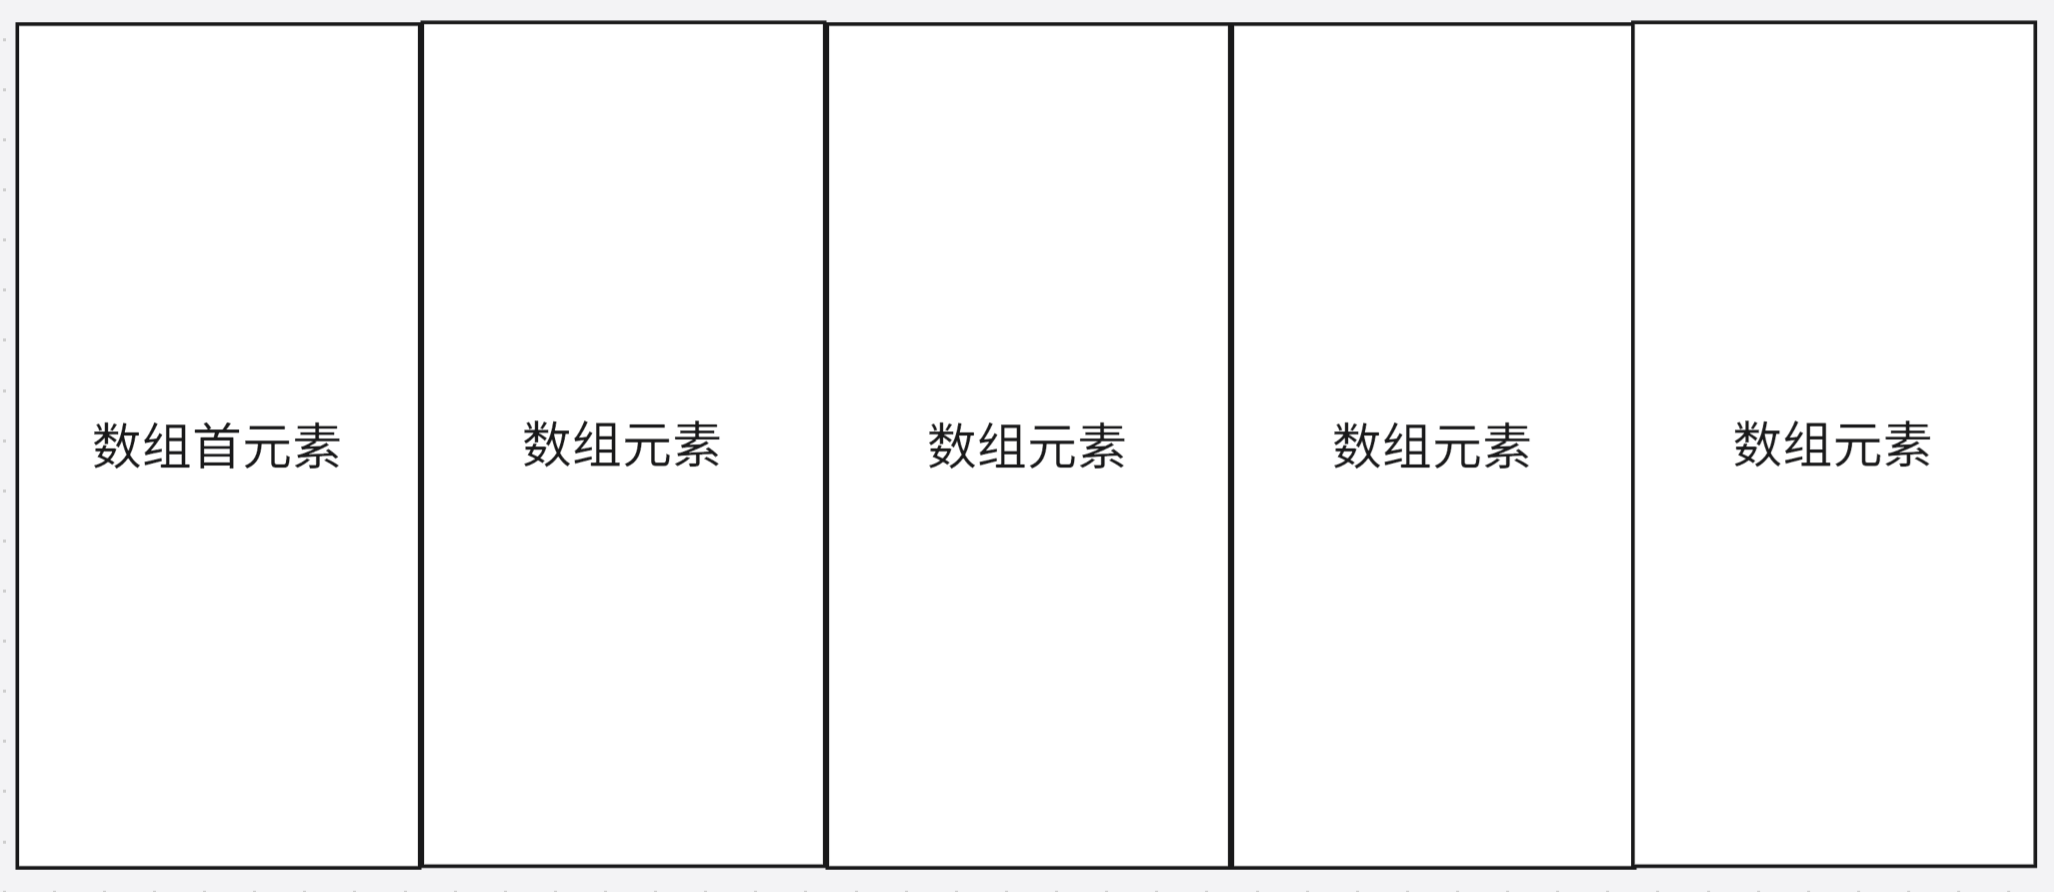
\includegraphics[width=0.7\textwidth]{数组.png}
    \caption{数组} % 图片标题
    \label{fig:数组} % 图片标签,用于引用
\end{figure}

\textbf{数组(Array)},又称\textbf{顺序表},它的STL容器有两种,分别是$array$和$vector$。

$array$是固定大小的数组。$vector$是一种动态数组,可以动态增长,可以根据需要自动分配内存。两者的声明方式如下:
\begin{tcode}
std::array<int,5> arr;
std::vector<int> vec;
\end{tcode}

$array$并不常用,因为它是固定大小的,如果需要改变大小,只能重新声明一个新的数组。
可以参考这篇blog详细了解:

\url{https://blog.csdn.net/qq_38410730/article/details/102802239}

$vector$由于其动态性,可以根据需要自动分配内存,因此使用起来比较方便,在工程实践中也更常用。
$vector$的实现原理是当检测到$vector$的容量不足时,会自动分配新的内存(原来的大小$\times$2),并将原有数据复制到新内存中。
这个复制的过程非常缓慢,因此,在使用大型的资源时,$vector$的效率可能会比较低。

成员函数(常用部分):
\begin{tcode}
std::vector<int> vec{1,2,3,4,5,6};
vec[0];         //访问(快速)
vec.at(0);    //访问(安全)
vec.front();    //第一个元素
vec.back();     //最后一个元素
vec.empty();    //检查是否为空
vec.size();     //返回容器大小
vec.reserve(10);//预留空间
vec.clear();    //清除所有元素
vec.insert(vec.begin(),1);//插入元素
vec.erase(vec.begin());//删除元素
vec.push_back(1); //在最后添加
vec.emplace_back(); //在最后添加
vec.pop_back();     //删除最后一个
\end{tcode}

\textbf{链表(List)}:链表是一种非连续的内存块,它是由一系列节点组成,每个节点都包含数据和指针。
链表的实现原理是每个节点都包含一个指针,指向下一个节点。链表的头节点称为头指针,尾节点称为尾指针。
链表的插入、删除操作都比较容易,只需要改变指针即可,但是查找操作比较麻烦,需要从头节点开始遍历。
\begin{figure}[H]
    \centering
    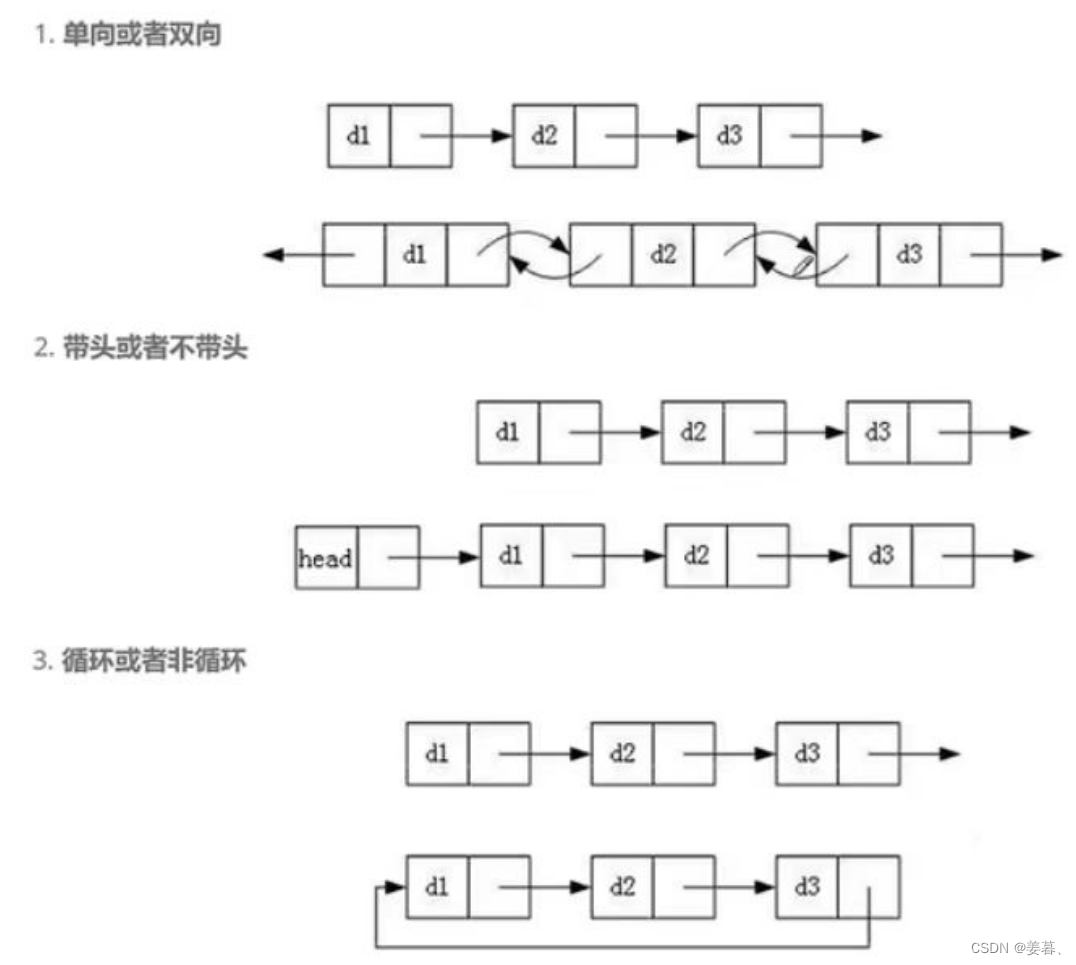
\includegraphics[width=0.7\textwidth]{链表1.png}
    \caption{链表} % 图片标题
    \label{fig:链表} % 图片标签,用于引用
\end{figure}

它的STL容器是$list$(双向链表)和$forward\_list$(单向链表)。比较简单,请自行去查阅相关文档:

\url{https://zh.cppreference.com/w/cpp/container/list}

\textbf{队列(Queue)}:队列是一种线性数据结构,它按照\textbf{先进先出}的原则进行操作。队列有两个基本操作,分别是\textbf{入队}和\textbf{出队}。入队操作是在队列的末尾添加一个元素,而出队操作是从队列的头部移除一个元素。队列有两个端点,队头和队尾,队头是队列的第一个元素,出队操作发生的地方,队尾是队列的最后一个元素,入队操作发生的地方。通常情况下,\textbf{不允许随机访问}队列中的元素,只能访问队头元素。
队列在\textbf{多任务处理、打印任务管理、缓冲处理}等场景中有广泛应用,它帮助维持操作的顺序和流程控制。
(很常用)
\begin{figure}[H]
    \centering
    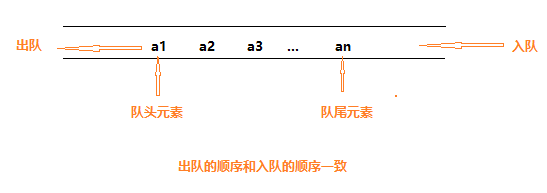
\includegraphics[width=0.7\textwidth]{队列1.png}
    \caption{入队和出队操作} % 图片标题
    \label{fig:入队和出队操作} % 图片标签,用于引用
\end{figure}
\begin{figure}[H]
    \centering
    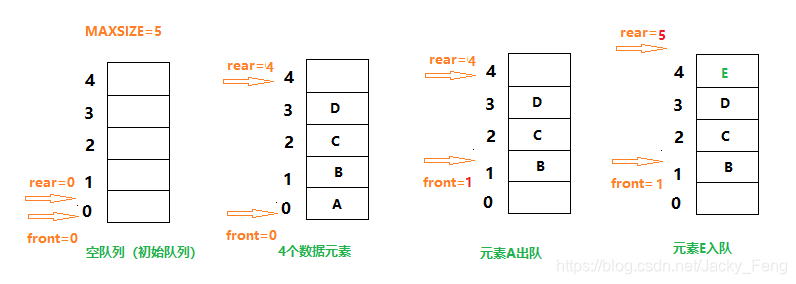
\includegraphics[width=0.7\textwidth]{队列2.png}
    \caption{队列实现方式} % 图片标题
    \label{fig:队列实现方式} % 图片标签,用于引用
\end{figure}

它的STL容器是$deque$,基于双向队列,C++还实现了3种容器适配器:
$stack$(堆栈),$queue$(单向队列),$priority\_queue$(优先队列),相较于$deque$,我们更常用$queue$
进行队列操作。
具体用法,请自行查阅相关文档:

\url{https://zh.cppreference.com/w/cpp/container/deque}

\url{https://zh.cppreference.com/w/cpp/container/queue}

\textbf{优先队列(Priority Queue)}:优先队列是一种特殊的队列,它允许插队的出现,可以根据“重要性”对队中元素进行排序。
优先队列的实现原理是每个元素都有一个优先级,优先级越高,元素越容易被取出。
优先队列的应用场景有很多,如任务调度、排序、搜索等。

\begin{figure}[H]
    \centering
    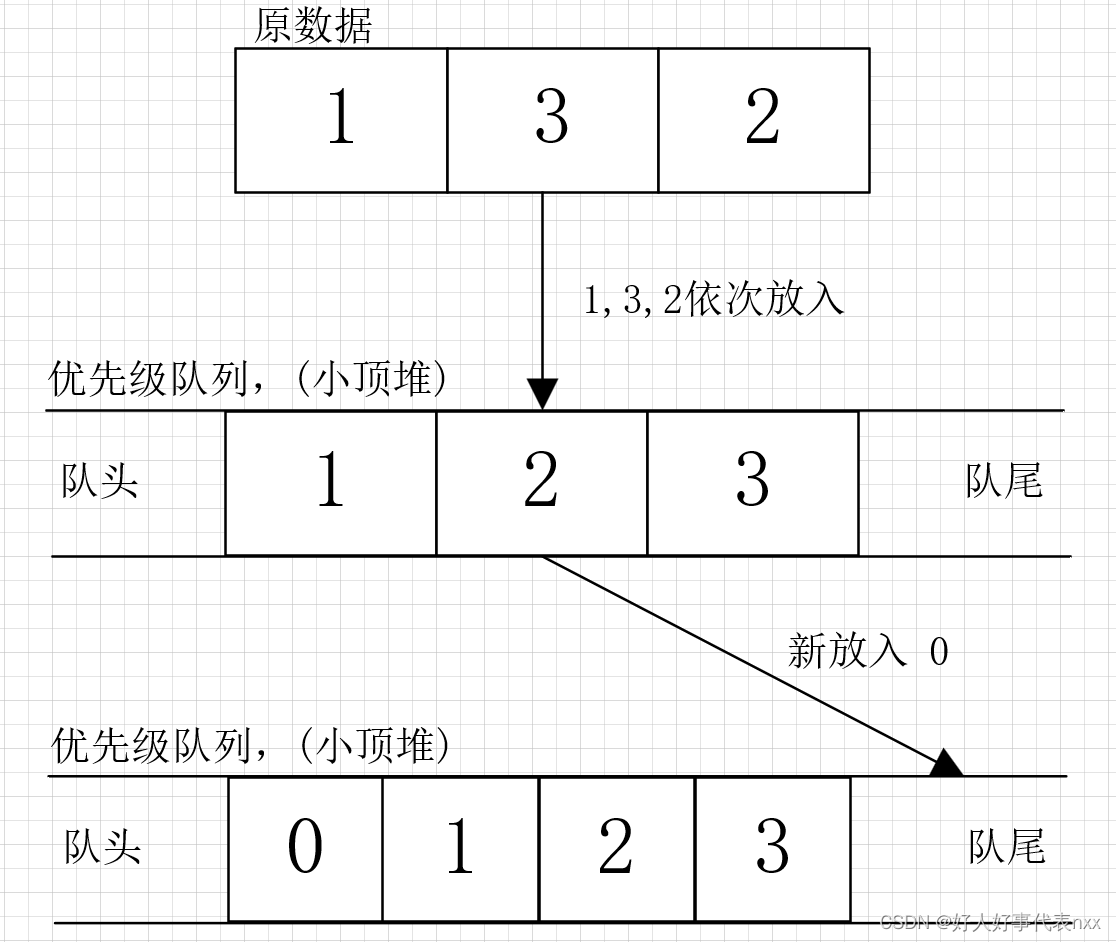
\includegraphics[width=0.7\textwidth]{优先队列1.png}
    \caption{优先队列} % 图片标题
    \label{fig:优先队列} % 图片标签,用于引用
\end{figure}

它的实现是容器适配器$priority\_queue$,
具体用法,请自行查阅相关文档:

\url{https://zh.cppreference.com/w/cpp/container/priority_queue}


\textbf{堆栈(Stack)}:堆栈是一种线性数据结构,它按照\textbf{先进后出}的原则进行操作。堆栈有两个基本操作,分别是\textbf{压栈}和\textbf{弹栈}。压栈操作是在堆栈的顶部添加一个元素,而弹栈操作是从堆栈的顶部移除一个元素。堆栈有两个端点,栈顶和栈底,栈顶是堆栈的顶部,压栈操作发生的地方,栈底是堆栈的底部,弹栈操作发生的地方。
堆栈在\textbf{函数调用、表达式求值、回溯、计算器、括号匹配、迷宫寻路}等场景中有广泛应用。

\begin{figure}[H]
    \centering
    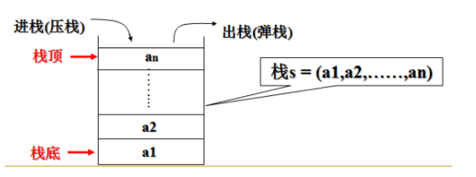
\includegraphics[width=0.7\textwidth]{堆栈1.png}
    \caption{压栈和弹栈操作} % 图片标题
    \label{fig:入队和出队操作} % 图片标签,用于引用
\end{figure}
\begin{figure}[H]
    \centering
    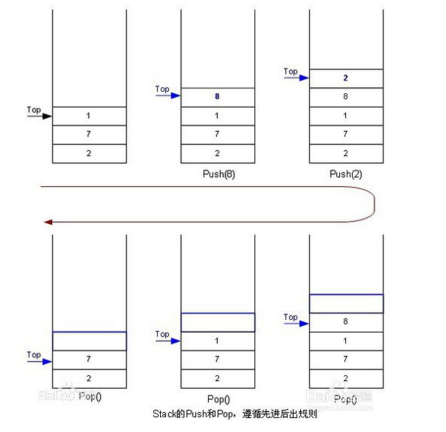
\includegraphics[width=0.7\textwidth]{堆栈2.png}
    \caption{堆栈实现方式} % 图片标题
    \label{fig:队列实现方式} % 图片标签,用于引用
\end{figure}

它的实现是容器适配器$stack$,
具体用法,请自行查阅相关文档。
\url{https://zh.cppreference.com/w/cpp/container/stack}

\textbf{树(Tree)}:树是一种非线性数据结构,它是由节点和边组成,节点之间存在着一种特定的关系。树的种类很多,如二叉树、二叉搜索树、AVL树、红黑树、B树、B+树、B*树等。
\begin{figure}[H]
    \centering
    \includegraphics[width=0.7\textwidth]{树1.png}
    \caption{树的逻辑图(了解即可)} % 图片标题
    \label{fig:队列实现方式} % 图片标签,用于引用
\end{figure}

\begin{figure}[H]
    \centering
    \includegraphics[width=0.7\textwidth]{树2.png}
    \caption{树的示意图} % 图片标题
    \label{fig:队列实现方式} % 图片标签,用于引用
\end{figure}

\textbf{堆(Heap)}:堆是一种特殊的树,它是一个\textbf{完全二叉树},即除叶节点外,其他的每个节点都有两个子节点。
每个节点都有一个值,并且每个节点\textbf{都大于或等于其子节点}(这是最大堆max-heap,类似的,还有最小堆min-heap)。堆的应用场景有很多,如排序、优先队列、图算法、堆排序等。

\begin{figure}[H]
    \centering
    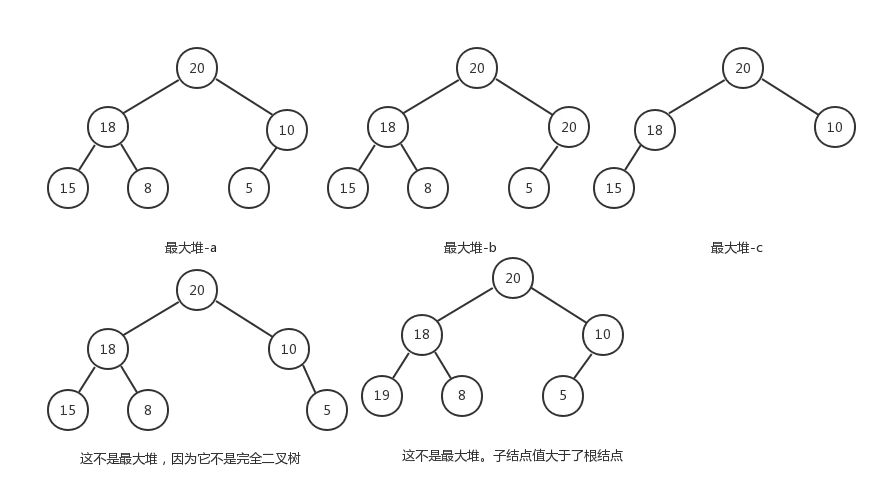
\includegraphics[width=0.7\textwidth]{最大堆.png}
    \caption{最大堆的示意图} % 图片标题
    \label{fig:最大堆} % 图片标签,用于引用
\end{figure}

\begin{figure}[H]
    \centering
    \includegraphics[width=0.7\textwidth]{堆1.png}
    \caption{最大堆和最小堆} % 图片标题
    \label{fig:最大堆和最小堆} % 图片标签,用于引用
\end{figure}

优先队列就是根据这个原理实现的,它是一种特殊的堆,具有\textbf{快速查找}的特性。他通过对于每个任务的重要程度进行编号,并将编号大的任务放在堆的顶部,这样就可以快速的找到重要的任务。
由于堆的排序算法非常快,可以实现更快速的任务调整,因此优先队列被广泛地应用于\textbf{任务管理}中。

优先队列的STL容器是$priority\_queue$。

具体用法,请自行查阅相关文档:

\url{https://zh.cppreference.com/w/cpp/container/priority_queue}

\textbf{映射(Map)}:映射是一种关联容器,它是一个\textbf{键值对}的集合,其中每个键都是唯一的,值可以重复。
映射的实现原理是通过哈希表(或红黑树)实现的,因此,查找、插入、删除操作的时间复杂度都是$O(1)$(或$O(logN)$)。

\textbf{红黑树(Red-Black Tree)}是一种随机查找速度比较快的\textbf{平衡二叉树}\footnote{
    平衡二叉树,也叫AVL树,它或者是一颗空树,或者具有以下性质的二叉排序树:它的左子树和左子树的高度之差(平衡因子)的绝对值不超过1,且它的左子树和右子树都是一颗平衡二叉树}
,他的查找、插入、删除操作的时间复杂度都是$O(logN)$ \footnote{
    O(logN)表示时间复杂度,N是问题的规模,O表示运行消耗时间的上界
}。

\textbf{哈希表(HashTable)}是一种\textbf{散列表},它通过\textbf{哈希函数}将键映射到值。
由于其使用计算来查找,因此,查找操作的时间复杂度都是$O(1)$
\footnote{常数的时间复杂度意味着不管问题的规模如何,
对于同一个长度的HashTable,算法的运行时间都不会随着问题的规模增加而增长。}。
但是哈希表的建立比较困难,需要消耗很多资源。
而且存储长度有限,当元素过多时,哈希表的性能会下降。当哈希表满时,需要执行\textbf{再散列(Rehashing)},解决\textbf{哈希冲突(Hash Collision)}问题,
这个过程需要消耗大量时间。

两者各有优劣,在实际应用中,需要根据具体问题选择。
红黑树型映射的STL容器是$map$,哈希表型映射的STL容器是$unordered\_map$,
具体用法,请自行查阅相关文档:

\url{https://zh.cppreference.com/w/cpp/container/map}

\subsubsection{STL的迭代器}

\textbf{迭代器},是一种检查容器内元素并遍历元素的数据类型,通常用于对C++中各种容器内元素的访问,
但不同的容器有不同的迭代器,初学者可以将迭代器理解为一个可以\textbf{自动向后移动的指针}。

常用的可迭代的容器有:

\begin{enumerate}
    \item 序列容器:$array$、$vector$、$deque$、$list$、$forward\_list$等
    \item 关联容器:$set$、$map$、$multimap$等
\end{enumerate}

$queue$、$stack$、$priority\_queue$是容器适配器,必须满足一定规则,没有迭代器。

对于可迭代容器,一般可以使用.begin()和.end()方法获取迭代器,.begin()方法返回指向第一个元素的迭代器,
.end()方法返回指向最\textbf{后一个元素的迭代器的下一位置}。
使用迭代器,可以方便的对容器内元素进行遍历,例如:

\begin{tcode}
std::vector<int> vec{1,2,3,4,5,6,7,8,9,0};
for(auto it = vec.begin();it != vec.end();++it){
    std::cout << *it << std::endl;
}
\end{tcode}

也可以简写为:

\begin{tcode}
for (auto it: vec) {
    std::cout << it << std::endl;
}
\end{tcode}

还可以使用迭代器对容器内元素进行修改,例如:

\begin{tcode}
std::vector<int> vec{1, 2, 3, 4, 5, 6, 7, 8, 9, 0};
vec.erase(vec.begin()+5);//删除第6个元素
vec.erase(vec.begin()+5,vec.end());//删除第6个元素之后的所有

std::vector<int> vec1{1, 2, 3, 4, 5, 6, 7, 8, 9, 0};
std::iter_swap(vec1.begin(),vec1.begin()+1);//交换第一个和第二个元素

std::vector<int> vec2{1, 2, 3, 4, 5, 6, 7, 8, 9, 0};
//此函数需要头文件<algorithm>
std::sort(vec2.begin(),vec2.end(),[](int& a,int& b){
    return a>=b;
});

//此函数需要头文件<algorithm>
//删除大于5的元素
auto newVec = std::remove_if(vec2.begin(),vec2.end(),[](int& a){
    return a>5;
});
\end{tcode}

我们不会使用十分复杂的迭代器,感兴趣的同学可以看一下cppreference的相关文档:

\url{https://zh.cppreference.com/w/cpp/iterator}

\textbf{迭代器失效}:迭代器失效指的是迭代器因为某些操作而不再指向原来的元素,
或者不再保持有效的状态,这样的迭代器如果继续使用,可能会导致未定义行为,包括程序崩溃。
通俗的理解就是,当你对容器进行了操作时,更改了容器的大小,但是迭代器仍然指向原来的位置,
这样就会导致读取错误的内存,这就是迭代器失效。

\begin{tcode}
std::vector<int> vec={1,2,3,4,5,6,7,8,9,10};
for(auto it = vec.begin(); it!= vec.end(); ++it){
    if(*it%2==0){
        vec.erase(it);
    }
}
\end{tcode}

看上面的代码,当执行到vec.erase(it)时,it已经失效,因为执行了erase之后,
vec的大小发生了变化,这导致了迭代器失效。

在实践过程中, 在下面的几种情况下,迭代器会失效,需要\textbf{避免}出现:
\begin{enumerate}
    \item 当执行erase方法时,指向删除节点的迭代器全部失效,指向删除节点之后的全部迭代器也失效
    \item 当进行push\_back\(\)方法时,end操作返回的迭代器肯定失效。
    \item 当插入\(push_back\)一个元素后,capacity返回值与没有插入元素之前相比有改变,
    则需要重新加载整个容器,此时first和end操作返回的迭代器都会失效。
    \item 当插入\(push_back\)一个元素后,如果空间未重新分配,指向插入位置之前的元素的迭代器仍然有效,但指向插入位置之后元素的迭代器全部失效。
\end{enumerate}

对于关联容器,使用迭代器时,删除一个键值对知识当前这个迭代器失效,别的迭代器不会受到影响,
这可能是由于底层使用红黑树实现的原因,但是实际应用中,仍然不应该冒这个风险,因此,
必须\textbf{坚决避免迭代器失效问题的发生}。

在具体的应用中,我们在使用迭代器遍历时,应该注意不要对容器进行增删操作,更不应该改变容器的大小。
可以将不需要的元素放在\textbf{容器的末尾}或者\textbf{记录下需要删除的迭代器},然后适时删除。例如:

\begin{tcode}
for(auto it = vec.begin(); it!= vec.end(); ++it){
    if((*it)%2==0){
        its.push_back(it-vec.begin());
    }
}

int i=0;
for(auto it : its){
    vec.erase(vec.begin()+it-i);
    i++;
}
}
\end{tcode}

这种方法,非常\textbf{不优雅},因此,\textbf{不要使用}。

\textbf{更多的用法等待着同学们自己去探索!}

\subsubsection{系统级内存运行逻辑}

C++是一个十分灵活的编程语言,其中指针的概念为程序员们提供了直接操纵内存的能力。
指针的使用使得程序员可以自由的操作内存,但是也带来了一些安全性和复杂性问题。
因此,了解程序运行的底层逻辑,对于理解C++至关重要,对于提高程序效率举重若轻,下面我们来看看C++的内存运行逻辑。

\begin{figure}[H]
    \centering
    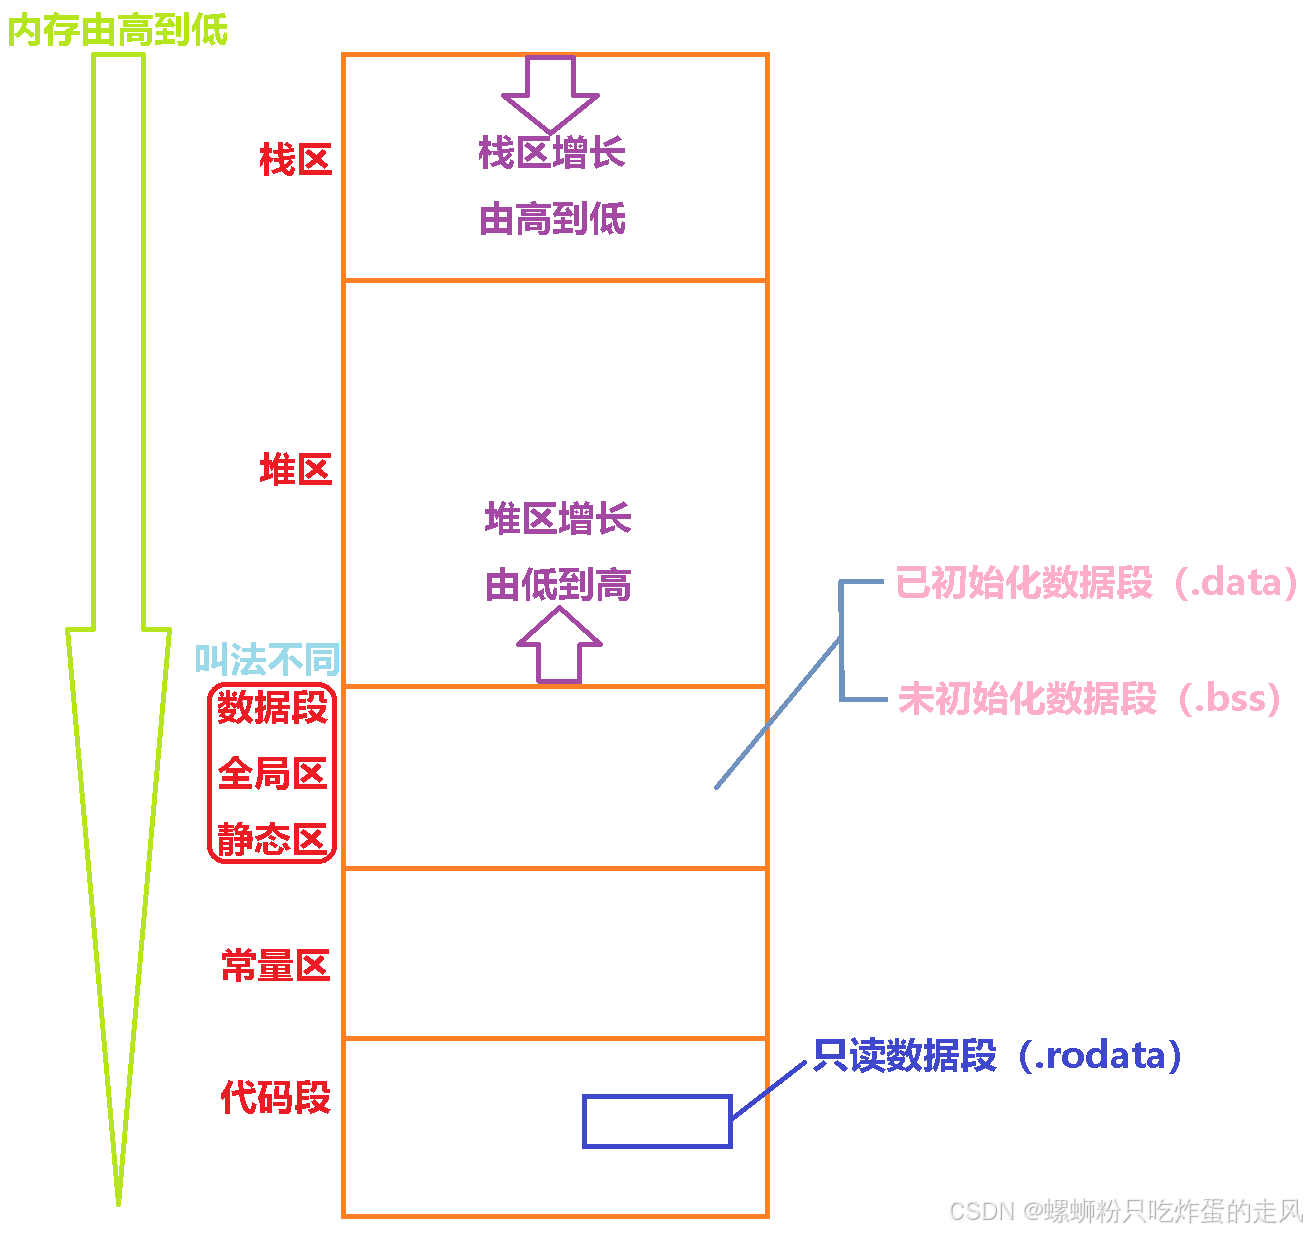
\includegraphics[width=0.7\textwidth]{系统内存.png}
    \caption{系统内存分区} % 图片标题
    \label{fig:内存分区} % 图片标签,用于引用
\end{figure}

如图\ref{fig:内存分区},系统内存分为\textbf{代码区、常量区、全局/静态变量区、堆区、栈区等几个部分}。

\textbf{代码区和常量区}是存放程序代码和常量数据的区间一般不作区分,这里的数据是只读的,其中存储着一些在编译过程前就可以确定的数据内容
,如代码、$constexpr$修饰的变量、$const$修饰的在预编译期可以确定的值等,
一些字面常量如"Hello World!",也存储于其中。程序在常量区中只能读取数据。

\textbf{全局/静态变量区}是存放全局/静态变量的区间,全局变量在程序运行前就已经分配了内存,静态变量在程序运行前也已经分配了内存。
但是静态变量的生命周期比全局变量长,它在程序运行结束后才释放内存。

\begin{enumerate}
    \item 全局变量:在函数外部定义的变量,它们具有全局作用域。
    \item 静态全局变量:在函数外部定义并用 $static$ 关键字修饰的变量,它们具有内部链接属性,即它们只能在定义它们的文件内部可见。
    \item 静态局部变量:在函数内部定义并用 $static$ 关键字修饰的变量,它们在函数调用结束后仍然存在,并且保持它们的值。
    \item 类静态成员变量:在类定义中使用 $static$ 关键字声明的成员变量,它们属于类而不是类的任何一个实例。
\end{enumerate}

解释一下\textbf{静态}:
\begin{enumerate}
    \item 生命周期上,静态变量在程序开始运行前或类的实例化之前就已经分配了内存,在程序运行结束后才释放内存。地址不会发生变化,就静静“躺”在静态变量区,直到程序结束。
    \item 相对于$new$的动态分配,可以让程序员选择什么时候分配和释放内存,而$static$变量则是一直存在的,直到程序结束。
    \item 静态全局变量也具有全局作用域,他与全局变量的区别在于如果程序包含多个文件的话,他作用于定义它的文件里,不能作用到其他文件里,即被$static$关键字修饰过的变量具有文件作用域。这样即使两个不同的源文件都定义了相同的静态全局变量,他们也是不同的变量。这点于全局变量不同。
\end{enumerate}

\textbf{堆区}:堆区是由程序员手动分配和释放的内存,堆区的分配和释放由\textbf{程序员控制},程序员可以通过$new$和$delete$操作符来分配和释放内存。

在大小上,堆区的大小相对于栈区是很大的,因此可以存储更多的数据。初次之外,堆区是由程序员全权负责管理的,程序员必须小心管理堆区的分配和释放,确保程序的正确性和安全性,一般使用\textbf{智能指针}和$nullptr$判断提高程序的稳定性。
但与此同时,堆区也提供了更为灵活的编程和数据传递模式,可以参考下面的例子:
\begin{tcode}
std::vector<int>* func(){
    std::vector<int>* a = new std::vector<int>({1,2,3,4});
    std::vector<int> b{1,2,3,4};
    return a;//return &b;
    //换成return &b;之后再试试呢?
}

int main() {
    auto vecPtr = func();
    return 0;
}
\end{tcode}

\textbf{栈区}:栈区是由\textbf{编译器自动分配和释放的内存},栈区的分配和释放都是编译器\textbf{自动完成}的,程序员\textbf{无法直接控制}栈区的分配和释放。
栈区存储数据的优势在于\textbf{快速},但是也有一些缺点,比如栈区的大小是有限的,因此在函数调用层次过深时,可能会出现栈溢出。
栈区的大小一般是$2MB$,因此栈区的大小是有限制的,如果函数调用层次过深,可能会出现栈溢出。

\textbf{系统内存管理}:系统内存管理是操作系统的工作,它负责分配和释放系统内存,其中操作系统会自行决定栈内存,下面我们讨论一下栈区的操作。

在栈内存中,数据存储在系统栈中,只有一个开口,数据只能从栈顶入栈和出栈。在切换代码的\textbf{作用域}时,上一个作用域的数据会被新的数据压在栈的下方,
这些数据将不能被当前的程序进程所读取,直到当前的这些数据被弹出栈。
栈内存的设计是十分精妙的,它可以有效的解决内存分配和释放的问题,亦可以实现函数的层次调用,作为一名C++程序员,我们要理解透彻栈内存的运行逻辑。

\textbf{函数递归的底层原理}:函数递归是一种非常有趣的编程技巧,它可以让程序员以一种\textbf{迭代}的思想来理解和编写代码。

\begin{figure}[H]
    \centering
    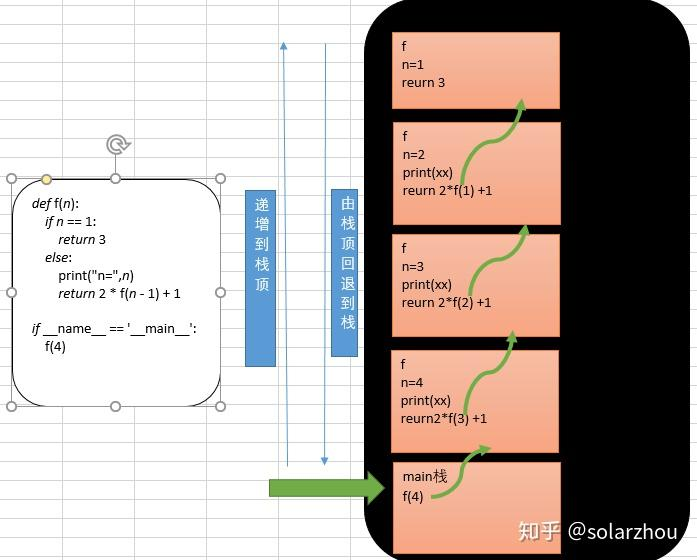
\includegraphics[width=0.7\textwidth]{栈递归.jpg}
    \caption{函数递归调用栈} % 图片标题
    \label{fig:栈递归} % 图片标签,用于引用
\end{figure}

在函数调用时,新的函数的栈帧会被压入栈中(称为栈帧),从而覆盖掉原来的\textbf{栈帧},当函数返回时,栈帧会被弹出栈。
露出原来的函数栈帧。当函数调用自身时,会形成一个\textbf{递归调用栈}。

需要注意的是,栈内存的大小是有限制的,当函数调用层次过深时,会出现栈溢出。

\subsubsection{C++的多线程}

多线程技术是C++中非常重要的特性之一,它可以让程序员以更高的并发性和速度运行程序。使用多线程可以提高程序的运行效率,丰富程序的运行逻辑,实现许多单线程所不能实现的功能。
在C++中,提供了$<threaed>$库来实现多线程的功能。

\textbf{多线程的原理}:多线程是指在同一程序中同时运行多个线程来完成不同的任务,以提高资源利用率和程序响应速度。
硬件条件上,多线程需要CPU支持多核处理或多任务处理,以及足够的内存和处理器资源。在多线程编程过程中,可能遇到一些问题,
包括线程同步、死锁、竞态条件等,这些问题可能导致程序运行不稳定、性能下降甚至系统崩溃。
因此,在设计多线程程序时,需要充分考虑线程之间的\textbf{协作与互斥},合理分配资源,以保障程序的正确性和高效性。
在多线程之中,有两种主要的设计模式,即\textbf{阻塞}和\textbf{非阻塞}。

\begin{enumerate}
    \item \textbf{阻塞}:在阻塞模式下,线程在等待某个事件的发生,如等待IO操作完成、等待子进程结束等。
当某个事件发生时,线程会被唤醒,并开始执行。

    \item \textbf{非阻塞}:在非阻塞模式下,线程在等待某个事件的发生,但不会被挂起,而是继续执行后续代码。
当某个事件发生时,线程会被通知,并开始执行。
\end{enumerate}


\textbf{创建线程}:
C++11中引入的$<thread>$库提供了多线程的支持,它提供了$std::thread$类来创建和管理线程:

\begin{tcode}
用法:std::thread ThreadName(函数指针,[参数]);
实例:
void function1(){for(int i=0;i<1000;i++);}
void function2(int a,int &b){for(int i=0;i<1000;i++);}
int main() {
    std::thread th1(function1);
    int a=0, b=0;
    std::thread th1(function1,a,std::ref(b));
    return 0;
}
\end{tcode}

如果你想要在线程中传递参数,可以直接传递参数,也可以使用引用传递参数,引用传参的时候需要使用$std::ref()$函数。
你也可以使用$join()$方法使主线程等待所有线程结束,
$detach()$方法将线程分离,这样主线程就不会等待主线程结束而结束。

\textbf{线程同步和互斥锁}:
多线程程序的稳定性和互斥锁是多线程编程中经常遇到的问题。请参考下面的例子:
\begin{tcode}
int i=0;
void function1(){
    for(int j=0;j<100000;j++)
        i++;
}

int main() {
    std::thread th1(function1);
    for(int j=0;j<100000;j++)
        i++;
    if(th1.joinable())
        th1.join();
    std::cout << i;
    return 0;
}
\end{tcode}
在程序的运行过程中,$i$的值可能是$0$,也可能是$200000$,这取决于线程的调度。
当两个线程同时拿到$i$的地址时,同时对i进行写入操作,两者就会出现线程同步问题。
那怎么解决这个问题呢?$std::mutex$和$std::lock\_guard$为我们提供了解决方案——互斥锁。是解决线程同步问题的两种方法。
$mutex$是一种同步机制,它可以保证同一时刻只有一个线程对共享资源进行访问。
$lock\_guard$是一个智能指针,它可以自动获取互斥锁,并在离开作用域时自动释放互斥锁。

\begin{tcode}
#include <iostream>
#include <thread>
#include <mutex>

int i=0;
std::mutex lock;
void function1(){
    for(int j=0;j<100000;j++){
        lock.lock();
        i++;
        lock.unlock();
    }
}

int main() {
    std::thread th1(function1);
    for(int j=0;j<100000;j++){
        lock.lock();
        i++;
        lock.unlock();
    }
    if(th1.joinable())
        th1.join();
    std::cout << i;
    return 0;
}
\end{tcode}
发现程序的稳定性已经得到提高,在多次运行过程中,$i$的值始终是$200000$。这一点在多线程编程过程中非常重要,是所有程序员的必修课。
但是,这是又产生了一个新的问题,那就是程序员还是需要进行互斥锁的手动管理,这无疑会降低程序开发的效率。
类似于智能指针的,C++11中引入了$std::lock\_guard$来自动管理互斥锁,它可以自动获取互斥锁,并在离开作用域时自动释放互斥锁。

\begin{tcode}
#include <iostream>
#include <thread>
#include <mutex>

int i=0;
std::mutex lock;
void function1(){
    for(int j=0;j<100000;j++){
        std::unique_lock<std::mutex> Autolock;
        i++;
    }

}

int main() {
    std::thread th1(function1);
    for(int j=0;j<100000;j++){
        std::unique_lock<std::mutex> Autolock;
        i++;
    }

    if(th1.joinable())
        th1.join();
    std::cout << i;
    return 0;
}
\end{tcode}
程序测试成功,$i$的值始终是$200000$。

\textbf{死锁}:在使用互斥锁的时候,如果多个线程都在\textbf{等待对方释放锁},就会出现死锁。请看下面的例子:

\begin{tcode}
int i=0;
std::mutex lock1;
std::mutex lock2;
void function1(){
    for(int j=0;j<100000;j++){
        lock1.lock();
        lock2.lock();
        i++;
        lock2.unlock();
        lock1.unlock();
    }
}

int main() {
    std::thread th1(function1);
    for(int j=0;j<100000;j++){
        lock2.lock();
        lock1.lock();
        i++;
        lock2.unlock();
        lock1.unlock();
    }

    if(th1.joinable())
        th1.join();
    std::cout << i;
    return 0;
}

\end{tcode}

在这个例子中,两个线程都在等待对方释放锁,导致死锁。在设计时,尽量使得不同的互斥锁以相同的顺序被获取和释放,可以降低死锁的概率。

\textbf{原子变量}:在C++11中,引入了原子类型$std::atomic$,它可以保证变量的原子性,即在读写操作时,其他线程只能看到该变量的\textbf{已修改}值。
使用这种方式,可以增强程序的可读性。原子变量也不需要使用互斥锁进行同步,它可以自动保证原子性。

\textbf{条件变量}:条件变量($Condition Variable$)是一种用于线程同步的机制,通常与互斥锁($Mutex$)一起使用。条件变量提供了一种线程间的通信机制,允许一个线程等待另一个线程满足某个条件后再继续执行。

我们通过一个例子来简单理解一下这个问题:

现在小明在一张桌子上放一个苹果,而旁边有一群蒙着眼睛的人,因为他们的眼睛被蒙着,
他们如果想拿到这个苹果,就会时不时来桌子前摸一摸看看桌子是否有苹果,并且谁来桌子前摸苹果是无序的,
这时的场面就很混乱,小明一看不行,于是小明就桌子上放了个铃铛,并且组织需要苹果的人排好队,
有苹果小明就会摇响铃铛,排在第一个的人就拿走苹果,然后如果还想要苹果就到队尾排队等待
。此时混乱的场面就显得井然有序了。在本故事中,小明就是操作系统,苹果就是临界资源,
一群蒙着眼睛都人就是多线程,铃铛就是条件变量,排队就是实现同步,摇响铃铛就是唤醒线程。

使用条件变量主要是因为它们提供了在多线程编程中一种有效的同步机制。
当多个线程需要\textbf{等待某个特定条件}成立才能继续执行时,条件变量就显得尤为重要。
通过条件变量,线程可以安全地进入等待状态,直到被其他线程显式地唤醒或满足等待的条件。
这有助于避免线程的\textbf{无谓轮询或忙等待},提高了系统的响应能力和效率。
\textbf{注意}:在使用条件变量时,必须确保与\textbf{互斥锁}一起使用,以\textbf{避免竞态条件}的发生。

下面介绍一下$condition\_variable$的用法:

调价变量的使用大致可以分为两个大的功能,即$notify$和$wait$。

\begin{tcode}
std::condition_variable condition;//声明
condition.notify_all();//通知所有等待线程
condition.notify_one();//通知第一个接收的等待线程

std::unique_lock<std::mutex> Lock(mtx);
condition.wait(Lock);//等待条件成立
condition.wait(Lock,[](){return true;});//等待条件和第二个参数同时为true
\end{tcode}

\textbf{消费者-生产者模型},是多线程编程中经常使用的模型。
生产者-消费者模型是指多个生产者线程和多个消费者线程之间通过一个共享的缓冲区进行通信。
生产者线程负责生产数据,并将其放入缓冲区;消费者线程则负责从缓冲区中取出数据进行消费。
生产者和消费者之间通过一个\textbf{条件变量}进行同步,以保证缓冲区中的数据不会被消费者线程消费完。

\begin{tcode}
#include<iostream>
#include<thread>
#include<mutex>
#include<condition_variable>
#include<queue>
#include<functional>

std::mutex lock;
std::condition_variable cv;
std::queue<std::function<void()>> taskQueue;
void consumer(){
    while(1){
        std::unique_lock<std::mutex> Lock(lock);
        cv.wait(Lock,[&](){
            return !taskQueue.empty();
        });
        auto task = taskQueue.front();
        task();
        taskQueue.pop();
        Lock.unlock();
    }
}

void producer(int i){
    auto func = [](int id){
        std::cout << "task" << id << " is running!" << std::endl;
    };
    std::function<void()> task = std::bind(func,i);
    {
        std::unique_lock<std::mutex> Lock(lock);
        taskQueue.push(task);
    }
    cv.notify_one();
    std::this_thread::sleep_for(std::chrono::seconds(1));
}

int main(int argc,char** argv){
    std::thread consumer_thread(consumer);
    for(int i=0;i<100;i++){
        producer(i);
    }

    if(consumer_thread.joinable())
        consumer_thread.join();
    return 0;
}
\end{tcode}

\textbf{线程池}:线程池是一种常用的技术,它可以提高程序的并发性,减少线程创建和销毁的开销,并可以有效的利用系统资源。
下面是一种线程池的实现方式,尝试一下把它看懂吧!

\begin{tcode}
#include <iostream>
#include <thread>
#include <mutex>
#include <condition_variable>
#include <functional>
#include <vector>
#include <queue>

class ThreadPool
{
private:
    std::vector<std::thread> threads;
    std::queue<std::function<void()>> tasks;
    std::mutex mtx;
    std::condition_variable condition;
    bool stop;

public:
    ThreadPool(int numThreads):stop(false) {
        for (int i = 0; i < numThreads; i++) {
            threads.emplace_back([this] {
                while (1) {
                    std::unique_lock<std::mutex> lock(mtx);
                    condition.wait(lock, [this] {
                        return !threads.empty() || stop;
                    });
                    if (stop && tasks.empty())
                        return;

                    auto task = std::move(tasks.front());
                    tasks.pop();
                    lock.unlock();
                    task();
                }
            });
        }

    }

    ~ThreadPool() {
        {
            std::unique_lock<std::mutex> lock(mtx);
            stop = true;
        }
        condition.notify_all();
        for (auto& iter : threads) {
            iter.join();
        }
    }

    template<class F, class ...Args>
    void enqueue(F&& f, Args&&... args) {
        std::function<void()> task =
                std::bind(std::forward<F>(f), std::forward<Args>(args)...);
        {
            std::unique_lock<std::mutex> lock(mtx);
            tasks.emplace(std::move(task));
        }
        condition.notify_one();
    }

};

int main() {
    ThreadPool Pool(4);
    for (int i = 0; i < 100; i++) {
        Pool.enqueue([i] {
            std::cout << "task" << i << "is running!" << std::endl;
            std::this_thread::sleep_for(std::chrono::seconds(1));
            std::cout << "task" << i << "has finished!" << std::endl;
        });
    }

    return 0;
}
\end{tcode}